\section{Integralen}

\subsection{Inleidend voorbeeld}
\begin{minipage}{.25\linewidth}
	\raggedright
	
\includegraphics[width=4cm]{6_afgeleiden_integralen/inputs/QR_Code_INLEIDENDVB_module6_2new}
\end{minipage}
\begin{minipage}{.7\linewidth}
	Zie filmpje MOOC.
\end{minipage}

\subsection{Primitieve functies en onbepaalde integralen}

Beschouw een re\"ele functie van \'e\'en re\"eel veranderlijke, bijvoorbeeld de functie:
\begin{equation*}
F(x) = x^3-3x^2+x-1.
\end{equation*}
Deze functie heeft als afgeleide:
\begin{equation*}
f(x) = \frac{dF(x)}{d} = 3x^2-6x+1.
\end{equation*}
Men zegt dat $F(x)$ een \textbf{stamfunctie} of een \textbf{primitieve functie} is van $f(x)$.

\begin{definitie}
Een primitieve functie $F(x)$ van een functie $f(x)$ is een willekeurige functie die als afgeleide naar $x$ $f(x)$  heeft:	
\begin{equation*}
F'(x)=DF(x)=f(x)
\end{equation*}
\end{definitie}

Het zoeken naar een primitieve functie van een functie is eigenlijk het omgekeerde van afleiden.

$F(x)$ is niet de enige functie die als afgeleide $f(x)$ heeft.

De functies:

\begin{eqnarray*}
F(x) &=& x^3-4x^2+x-1 \\
F(x) &=& x^3-4x^2+x+3 \\
F(x) &=& x^3-4x^2+x-2 \\
\end{eqnarray*}

Hebben allen als afgeleide:

\begin{equation*}
f(x) = 3x^2-8x+1
\end{equation*}

Functies die slechts een constante van elkaar verschillen, hebben immers allen dezelfde afgeleide. Omgekeerd kan men ook aantonen dat functies die dezelfde afgeleide hebben op een interval $I$ een constant verschil op dat interval $I$ hebben.

\begin{definitie}
De verzameling van alle primitieve functies van $f(x)$ noemt men de onbepaalde integraal van $f(x)$. 
Als $F(x)$ een primitieve functie van $f(x)$ is dan schrijft men:
\begin{equation*}
\int f(x)dx = F(x) + C
\end{equation*}
Terminologie:
\begin{eqnarray*}
\int && \text{Het integraalteken} \\
f(x) && \text{De integrand (de te integreren functie)} \\
dx && \text{De differentiaal van de integratieveranderlijke} \\
C && \text{De integratieconstante }
\end{eqnarray*}
\end{definitie}

\subsection{Stelling van Newton Leibniz}
\begin{minipage}{.25\linewidth}
	\raggedright
	
\includegraphics[width=4cm]{6_afgeleiden_integralen/inputs/QR_Code_STNEWTONLEIBNIZ_module6_2new}
\end{minipage}
\begin{minipage}{.7\linewidth}
	Zie filmpje MOOC.
\end{minipage}

\subsection{Bijzondere onbepaalde integralen}

Iedere afgeleide van een bijzondere functie geeft aanleiding tot een bijzondere onbepaalde integraal.

\begin{voorbeeld} Omdat $D(\sin x)=\cos x$ is $\int \cos x dx = \sin x +C$.
\end{voorbeeld}

\begin{voorbeeld} Omdat $Dx^n=nx^{n-1}$ is $\int nx^{n-1}dx = x^n +C$.
	
Als je dit wat herwerkt bekom je $D \left( \frac{x^{m+1}}{m+1} \right) = x^m$ en dus $\int x^mdx=\frac{x^{m+1}}{m+1} + C$.
Deze onbepaalde integraal geldt voor alle $m \neq -1$.
Die laatste voorwaarde komt door de noemer $m+1$ die niet 0 mag zijn.
\end{voorbeeld}

\begin{voorbeeld} Omdat $D(\ln\vert x \vert)=\frac{1}{x}$ is $\int \frac{dx}{x} = \ln \vert x \vert +C$.
Vanwege $\frac{1}{x} = x^{-1}$ staat hier ook een uitkomst voor $\int x^m dx$ als $m=-1$, namelijk $\int x^{-1} dx = \ln \vert x \vert +C$.
\end{voorbeeld}

Op deze wijze ontstaat de volgende lijst van bijzondere onbepaalde integralen.

\begin{ftrekenregel}
	
\begin{equation*}
\int \dx = x + C
\end{equation*}
\begin{equation*}
\int x^n \dx= \frac{x^{n+1}}{n+1}+C \ (n \neq -1)
\end{equation*}
\begin{equation*}
\int \frac{\dx}{x} = \ln{|x|}  +C
\end{equation*}
\begin{equation*}
\int e^{x} \dx = e^{x} +C
\end{equation*}
\begin{equation*}
\int a^{x} \dx = \frac{a^x}{\ln a}+C
\end{equation*}
\begin{equation*}
\int  \sin{x} \dx = - \cos{x}+C
\end{equation*}
\begin{equation*}
\int \cos{x} \dx = \sin{x}+C
\end{equation*}
\begin{equation*}
\int \frac{1}{\cos^2{x}} \dx = \tan{x} + C
\end{equation*}
\begin{equation*}
\int \frac{1}{\sin^2{x}} \dx = -\cot{x} + C
\end{equation*}
\begin{equation*}
\int \sec^2{x} \dx = \int \frac{1}{\cos^2{x} \dx} = \tan{x} + C
\end{equation*}
\begin{equation*}
\int \csc ^2{x} \dx = \int \frac{1}{\sin^2{x}} \dx = - \cot{x}+C
\end{equation*}
\begin{equation*}
\int \frac{\dx}{1+x^2} = \arctan{x} + C
\end{equation*}
\begin{equation*}
\int \frac{\dx}{a^2+x^2} = \frac{1}{a} \arctan{\frac{x}{a}}+C
\end{equation*}
\begin{equation*}
\int \frac{\dx}{\sqrt{1-x^2}}=\arcsin{x}+C
\end{equation*}
\begin{equation*}
\int \frac{\dx}{\sqrt{a^2-x^2}}=\arcsin{\frac{x}{a}}+C
\end{equation*}		
\end{ftrekenregel}


\subsection{Eenvoudige rekenregels}

Uit $D(f+g)=Df+Dg$ bekom je

\begin{eigenschap} Onbepaalde integraal van een som : \\
\[\int (f(x)+g(x))dx = \int f(x)dx + \int g(x)dx \hfill\]
\end{eigenschap}

Uit $D(cf)=cDf$ ($c$ is een getal) bekom je

\begin{eigenschap} Onbepaalde integraal van een functie vermenigvuldigd met een constante :\\
\[\int cf(x)dx = c \int f(x)dx \hfill\]
\end{eigenschap}

Met behulp van deze eigenschappen kun je alle integralen van veeltermfuncties uitrekenen.

\begin{voorbeeld}
	\begin{eqnarray*}
	\int (7x^3-4x^2+9x+13)dx
	&=&\int 7x^3dx+\int -4x^2dx+\int 9xdx + \int 13dx \text{ (rekenregel som)}\\
	&=& 7\int x^3dx -4 \int x^2dx+9\int xdx + 13 \int dx \text{ (rekenregel product met c)}\\
	&=& \frac{7x^4}{4} -\frac{4x^3}{3} + \frac{9x^2}{2} +13 x+C \text{ ($\int x^n dx=\frac{x^{n+1}}{n+1}+C$)}\\
	\end{eqnarray*}
\end{voorbeeld}

\begin{voorbeeld} 
	\begin{eqnarray*}
	\int (x+2)^2 \dx &=& \int (x^2+4x+4)\dx \\
	&=& \int x^2 \dx + 4 \int x\dx +4 \int \dx \\
	&=& \frac{x^3}{3} + 4 \frac{x^2}{2} + 4x + C\\
	&=& \frac{x^3}{3} + 2 x^2 + 4x + C
	\end{eqnarray*}
\end{voorbeeld}

Algemener kun je onbepaalde integralen uitrekenen van de vorm zoals in het volgende voorbeeld.

\begin{voorbeeld}
	\begin{eqnarray*}
	\int (7\sqrt[3]{x^5}+\frac{2}{\sqrt[5]{x}}-\frac{3}{x})dx
	&=&\int (7x^{5/3}+2x^{-1/5}-\frac{3}{x})dx\\
	&=&7\int x^{5/3}dx+2\int x^{-1/5}dx-3\int \frac{dx}{x}\\
	&=& \frac{7x^{8/3}}{8/3}+\frac{2x^{4/5}}{4/5}-3\ln \vert x \vert +C\\
	&=& \frac{21\sqrt[3]{x^8}}{8}+\frac{5\sqrt[5]{x^4}}{2}-3 \ln \vert x \vert +C\\
	\end{eqnarray*}
\end{voorbeeld}

Sommige sommen zie je direct zoals in volgend voorbeeld

\begin{voorbeeld} 
	\begin{eqnarray*}
	\int (3 \sin x + 5 \cos x) \dx &=& 3 \int \sin x \dx + 5 \int \cos x \dx \\
	&=& 3 (-\cos x ) + 5 \sin x +C \\
	&=& -3 \cos x + 5 \sin x + C
	\end{eqnarray*}
\end{voorbeeld}

Andere sommen zie je niet zo direct zoals in volgend voorbeeld

\begin{voorbeeld}
	\begin{eqnarray*}
	\int \tan ^2 x dx
	&=&\int \frac{\sin^2 x}{cos ^2 x}dx\\
	&=& \int \frac{1-\cos^2 x}{\cos ^2 x} dx \text { (hoofdformule van goniometrie)}\\
	&=& \int \left( \frac{1}{\cos^2 x} -1 \right)dx\\
	&=& \int \frac{1}{\cos ^2 x} - \int dx\\
	&=& \tan x -x +C\\
	\end{eqnarray*}
\end{voorbeeld}

\subsection{Eenvoudige rekenregels - voorbeeld}
\begin{minipage}{.25\linewidth}
	\raggedright
	
\includegraphics[width=4cm]{6_afgeleiden_integralen/inputs/QR_Code_EENVRRVB_module6_2new}
\end{minipage}
\begin{minipage}{.7\linewidth}
	Zie filmpje MOOC.
\end{minipage}

\subsection{De bepaalde integraal}
Voor een functie $f$ continu en positief op een interval $I$ en $a$, $b$ binnen $I$ met $a<b$ noteren we $\int^b_a f(x)dx$ voor de oppervlakte van het vlakdeel begrensd door de $x$-as, de grafiek van $f$ en de verticale rechten $x=a$ en $y=b$.
(Je ziet die oppervlakte gearceerd in de figuur.)

%\gewonefiguur{width=.5\linewidth}{6_afgeleiden_integralen/inputs/2_7_fig1}

\begin{center}
	\tikzsetfigurename{module6_2_7_oppCurve}
\begin{tikzpicture}

\begin{axis}[xlabel=$x$,
ylabel=$y$,
axis lines = middle,
ticks=none]

\addplot[mark=none,color=white] {-1};

\addplot[name path=f,mark=none, domain=-5:5, samples=100,color=black] {2+x^2};
\addplot[mark=none, domain=-5:5, samples=100,color=white] {-5};

\path[name path=axis] (axis cs:0,0) -- (axis cs:4,0);

\addplot [
thick,
color=blue,
fill=blue, 
fill opacity=0.05
]
fill between[
of=f and axis,
soft clip={domain=2:4},
];

\node[below] at (axis cs: 2,0) {$a$};
\node[below] at (axis cs: 4,0) {$b$};

\end{axis}


\end{tikzpicture}
\end{center}


Algemener, als $f$ continu is op een interval $I$ en $a$, $b$ binnen $I$ met $a<b$ dan is $\int ^b_a f(x)dx$ gedefinieerd als de som van de oppervlakten tussen de $x$-as en de grafiek waar de functie $f$ positief is minus de som van de oppervlakten tussen de $x$-as en de grafiek waar de functie $f$ negatief is.
Een + op de volgende figuur duidt een oppervlakte aan die positief meetelt en een - duidt een oppervlakte aan die negatief meetelt.\\

%\gewonefiguur{height=8cm}{6_afgeleiden_integralen/inputs/2_7_fig2}

\begin{center}
	\tikzsetfigurename{module6_2_7_posneg}
\begin{tikzpicture}

\begin{axis}[xlabel=$x$,
ylabel=$y$,
axis y line = middle,
axis x line = middle]

\addplot[mark=none,color=white] {-1};
\addplot[name path=f,mark=none, domain=-2.5:2.5, samples=100,color=black] {x^4-5*x^2+2};

\node at (axis cs: -1.5,-2) {$-$};
\node at (axis cs: 0.3,1) {$+$};
\node at (axis cs: 1.5,-2) {$-$};
\node at (axis cs: 2.4,1) {$+$};

\draw [dashed,help lines] (-2,0) -| (-2,-2);
\draw [dashed,help lines] (2.5,0) -| (2.5,9.81);

\end{axis}


\end{tikzpicture}
\end{center}


%\begin{figure}[h]
%	\begin{center}
%		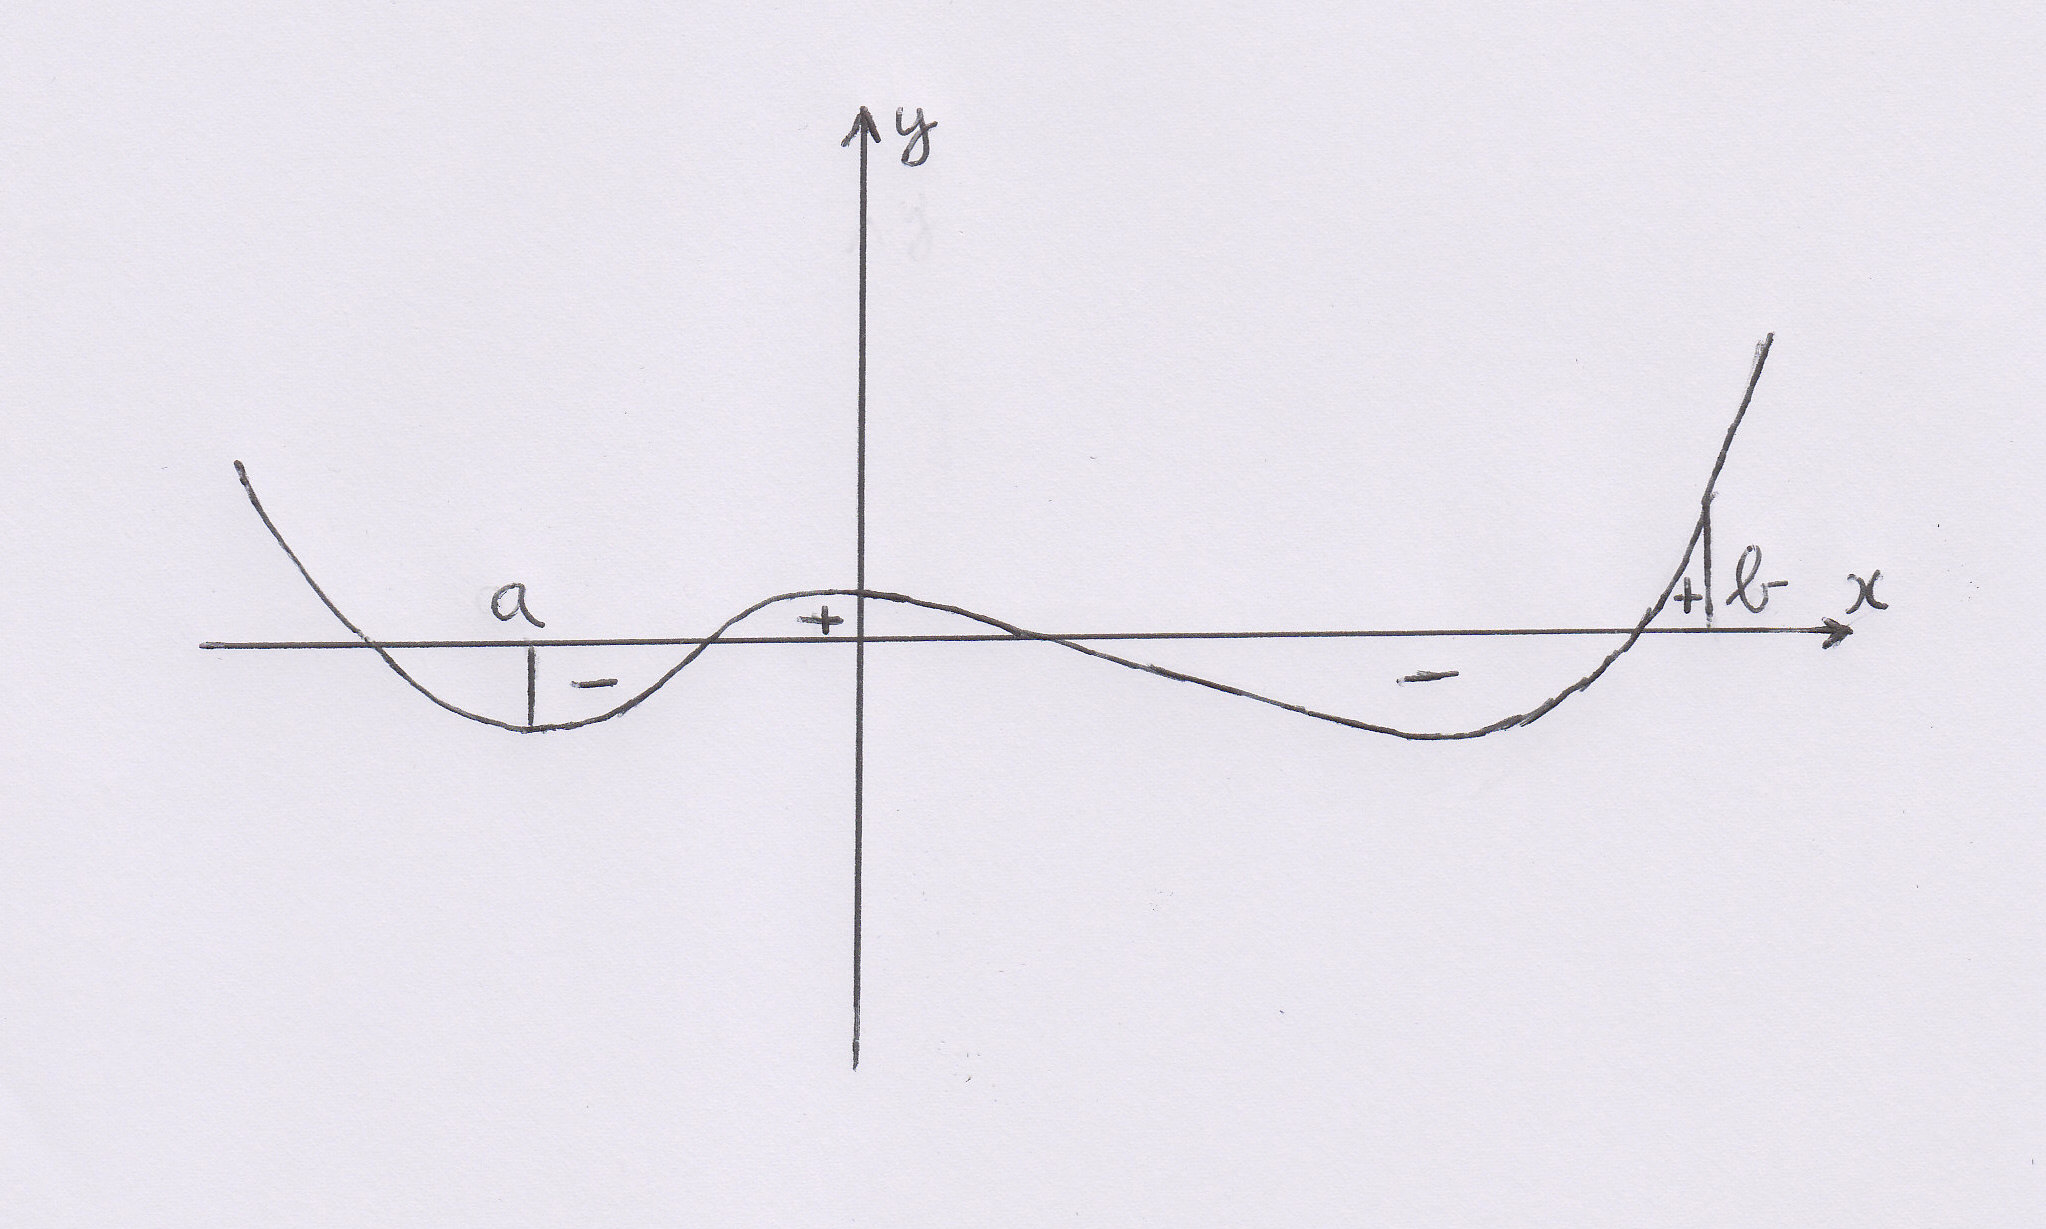
\includegraphics[height=5 cm]{6_afgeleiden_integralen/inputs/integraal2.JPG}
%		\caption{Bepaalde integralen: oppervlakten die positief en negatief meetellen.}
%		\label{fig:int:2}
%	\end{center}
%\end{figure}

Nog algemener, als $f$ continu is op een interval $I$ en $a$ en $b$ binnen $I$ dan is $\int ^b_a f(x)dx$

\hspace{1cm} reeds gedefinieerd als $a<b$

\hspace{1cm} $-\int^a_b f(x)dx$ als $a>b$

\hspace{1cm} 0 als $a=b$.\\

Je noemt $\int^b_a f(x)dx$ de bepaalde integraal van de functie $f$ van $a$ naar $b$.\\

Dank zij de volgende eigenschap kun je bepaalde integralen uitrekenen door middel van onbepaalde integralen.

\begin{eigenschap} Als $f$ een continue functie is op een interval $I$ en $F$ is een primitieve functie van $f$ dan geldt voor elementen $a$ en $b$ van $I$ dat\\
\[\int^b_a f(x)dx = F(b)-F(a)\]
\end{eigenschap}

Vorige eigenschap is een gevolg van de belangrijke stelling van Newton-Leibnitz die volgend verband geeft tussen afgeleiden en bepaalde integralen.

\begin{eigenschap}
	Als $f$ een functie is continu op een interval $I$ en $a$ is een element van $I$ dan voldoet de functie $F(x) = \int^x_a f(t)dt$ aan $DF(x)=f(x)$ voor alle $x$ in $I$.
\end{eigenschap}

Deze stelling van Newton-Leibnitz wordt aan de hand van een filmpje getoond in een voorbeeld.

%In het filmpje wordt de functie met voorschrift $f(x)=x$ gebruikt. De bijbehorende functie $F(x)$ wordt nu $O(x)$ genoteerd (misschien toch beter met $F(x)$ noteren) en is dus gegeven door de formule rechts bovenaan ($O(x)=\int ^x_0 tdt$).
%Voor de gegeven functie $f(x)=x$ is dit de oppervlakte getekend rechts bovenaan.
%
%De drie volgende tekeningen is de situatie voor een aantal waarden van $x$. Als je $x$ opeenvolgend $1$; $2$ en $\frac {1}{2}$ neemt dan bekom je telkens links de bijbehorende oppervlakte die elementair uit te rekenen is (oppervlakte van een driehoek). Rechts staat dan de berekening van die oppervlakte en dat geeft aanleiding tot een punt van de grafiek van die functie $O(x)$. De linkse tekening zijn dus steeds nieuwe tekeningen en de rechtse tekening is een punt meer van de grafiek van $O(x)$.
%
%Op de volgende bladzijde staat dan de berekening voor een willekeurige $x$ , krijg je daardoor het voorschrift van de volledige functie $O(x)$ en de grafiek ervan.
%
%Op de volgende lijn staat dan rechts de afgeleide van die functie $O(x)$ berekend en als je van die afgeleide dan links de grafiek tekent krijg je terug $f(x)=x$, de functie waarmee je startte.
%
%De tekst onderaan geeft terug de formulering van de stelling van Newton-Leibnitz en voor welke functie dat in het filmpje geïllustreerd is.
%
%In de SPOC was het de bedoeling dit zonder bijkomende woorden of tekst te maken, misschien is het in de MOOC toch beter om er tekst en/of geluid bij te plaatsen.
%
%Het is gewoon een idee om een fundamentele stelling uit de wiskunde door middel van een eenvoudig voorbeeld te illustreren. 


\subsection{De bepaalde integraal - voorbeeld}
\begin{minipage}{.25\linewidth}
	\raggedright
	
\includegraphics[width=4cm]{6_afgeleiden_integralen/inputs/QR_Code_BEPINTVB_module6_2new}
\end{minipage}
\begin{minipage}{.7\linewidth}
	Zie filmpje MOOC.
\end{minipage}


\subsection{Berekenen van bepaalde integralen}

Uit het voorgaande weten we dat uit $\int f(x)dx=F(x)+C$ volgt dat $\int^b_a f(x)dx=F(b)-F(a)$ (onder voorwaarde dat $f$ continu is op een interval dat $a$ en $b$ bevat).

Hierbij maakt men vaak gebruik van de voorstellingswijze: 
\begin{equation*}
\int_{a}^{b} f(x) \dx = [F(x)]_a^b = F(b)-F(a)
\end{equation*}

\begin{voorbeeld}
	\begin{eqnarray*}
		\int_{0}^{\frac{\pi}{2}} \sin x \dx = [-\cos x]_{x=0}^{x=\frac{\pi}{2}}=-\cos \frac{\pi}{2}-\cos 0 = 0+1 = 1 \\
		\int_{1}^{3} 2x^2 \dx = 2\int_{1}^{3} x^2 \dx = [\frac{2x^3}{3}]_{x=1}^{x=3}=\frac{2.27}{3}-\frac{2-1}{3}=18-\frac{2}{3}=\frac{52}{3} \\
		\int_{-3}^{2} e^x \dx = [e^x]_{x=-3}^{x=2}=e^2-e^{-3}\approx 7.339...
	\end{eqnarray*}
\end{voorbeeld}

\emph{Opmerking}
Bij berekening van de bepaalde integraal, noteer je de onbepaalde integraal tussen vierkante haken. Aan de rechterkant schrijf je onderaan de ondergrens en bovenaan de bovengrens. De integratieconstante $C$ noteer je niet bij de berekening van de bepaalde integraal.

\begin{eigenschap} Bepaalde integraal van een som
\[\int^b_a (f(x)+g(x))dx = \int^b_a f(x)dx + \int^b_a g(x)dx\]
\end{eigenschap}

\begin{eigenschap} Bepaalde integraal van een functie vermenigvuldigd met een getal
	\[\int^b_a c.f(x)dx = c \int^b_a f(x)dx\]
\end{eigenschap}

\begin{eigenschap} Opsplitsing van grenzen van een bepaalde integraal
	\[\int^b_a f(x) dx = \int^c_a f(x)dx + \int^b_c f(x)dx\]
\end{eigenschap}

Uit de defintie volgen ook nog de volgende twee rekenregels:

\begin{rekenregel}
	\[\int^a_a f(x) dx = 0\]

\[\int^b_a f(x) dx = - \int^a_b f(x) dx\]
\end{rekenregel}

\begin{voorbeeld}
	\begin{eqnarray*}
	\int_{1}^{5} [4-(x-3)^2] \dx &=& \int_{1}^{5} 4 \dx - \int_{1}^{5} (x-3)^2 \dx \\
	&=& 4 \int_{1}^{5} \dx - \int_{1}^{5} (x^2-6x+9) \dx \\
	&=& 4 \int_{1}^{5} \dx - \int_{1}^{5} x^2 \dx +6 \int_{1}^{5} d\ dx - 9 \int_{1}^{5} \dx \\
	&=& 4[x]_{x=1}^{x=5}-[\frac{x^3}{3}]_{x=1}^{x=5}+6[\frac{x^2}{2}]_{x=1}^{x=5}-9[x]_{x=1}^{x=5} \\
	&=& 20-4-\frac{125}{3}+\frac{1}{3}+75-3-45+9 \\
	&=& 52 - \frac{124}{3} \\
	&=& \frac{156}{3} - \frac{124}{3} \\
	&=& \frac{32}{3} \\
	\end{eqnarray*}
\end{voorbeeld}


\subsection{Oppervlakte berekenen met bepaalde integralen - voorbeeld}
\begin{minipage}{.25\linewidth}
	\raggedright
	
\includegraphics[width=4cm]{6_afgeleiden_integralen/inputs/QR_Code_OPPBEPINT_module6_2new}
\end{minipage}
\begin{minipage}{.7\linewidth}
	Zie filmpje MOOC.
\end{minipage}


\subsection{Oppervlakte berekenen met bepaalde integralen}

\begin{voorbeeld}
Bereken de oppervlakte begrensd door $y=x^3-x$, $x=-1$, $x=2$ en de $x$-as, zie de figuur.

%\gewonefiguur{width=.7\linewidth}{6_afgeleiden_integralen/inputs/2_11_vb20}

\begin{center}
	\tikzsetfigurename{module6_2_11_vb}
\begin{tikzpicture}

\begin{axis}[xlabel=$x$,
ylabel=$y$,
axis y line = middle,
axis x line = middle]

\addplot[mark=none,color=white] {-1};
\addplot[name path=f,mark=none, domain=-2:2, samples=100,color=black] {x^3-x};

\addplot +[mark=none,dashed] coordinates {(2, -6) (2, 6)};
\addplot +[mark=none,dashed] coordinates {(-1, -6) (-1, 6)};

%\node at (axis cs: -1.5,-2) {$-$};
%\node at (axis cs: 0.3,1) {$+$};
%\node at (axis cs: 1.5,-2) {$-$};
%\node at (axis cs: 2.4,1) {$+$};

%\draw [dashed,help lines] (-2,0) -| (-2,-2);
%\draw [dashed,help lines] (2.5,0) -| (2.5,9.81);

\end{axis}


\end{tikzpicture}
\end{center}

Tekenonderzoek van de functie:

\begin{equation*}
y=x^3-x=x(x^2-1)=x(x-1)(x+1)
\end{equation*}

De nulwaarden zijn dus $0$, $-1$ en $1$. Het tekenverloop is
\begin{center}
	\begin{tabular}{c|ccccccc}
	$x$ & & -1 & & 0 & & 1 & \\
	\hline
	$x$ & - & - & -& 0 & + & + & + \\
	$x^2-2$ & + & 0 & -& - & - & 0 & + \\
	\hline 
	$y=x^3-x$ & - & 0 & +& 0 & - & 0 & + 
	\end{tabular}
\end{center}

\begin{eqnarray*}
S &=& \int_{-1}^{2}|x^3-x|\dx = \int_{-1}^{0}(x^3-x)\dx - \int_{0}^{1}(x^3-x)\dx - \int_{1}^{2}(x^3-x)\dx \\
&=& [\frac{x^4}{4}\frac{x^2}{2}]_{-1}^{0} - [\frac{x^4}{4}\frac{x^2}{2}]_{0}^{1} + [\frac{x^4}{4}\frac{x^2}{2}]_{1}^{2} \\
&=& 0 - (\frac{1}{4}-\frac{1}{2}) - (\frac{1}{4}-\frac{1}{2}) + 0 + (4-2) - (\frac{1}{4}-\frac{1}{2}) \\
&=& \frac{1}{4} + \frac{1}{4} + 2 + \frac{1}{4} \\
&=& \frac{11}{4}
\end{eqnarray*}

\end{voorbeeld}

Algemener, stel dat $f$ en $g$ twee functies zijn die allebei continu zijn op een interval $I$. Stel dat $a$ en $b$ tot $I$ behoren met $a<b$. Op figuur hieronder is de gearceerde oppervlakte de oppervlakte begrensd door de grafieken van $f(x)$ en $g(x)$ en de verticale rechten $x=a$ en $x=b$.

%\gewonefiguur{width=.7\linewidth}{6_afgeleiden_integralen/inputs/2_11_vb20_2}

\begin{center}
	\tikzsetfigurename{module6_2_11_vb2}
\begin{tikzpicture}

\begin{axis}[xlabel=$x$,
ylabel=$y$,
axis y line = middle,
axis x line = middle,
ticks=none]

\addplot[mark=none,color=white] {-3};
\addplot[name path=f,mark=none, domain=-2:2, samples=100,color=red] {x^5+4*(x-1)^2} node[below,pos=1] {$f$};
\addplot[name path=g,mark=none, domain=-2:2, samples=100,color=blue] {1/4*(x^5+4*(x-1)^2)+5} node[above,pos=1] {$g$};

\addplot [
thick,
color=blue,
fill=blue, 
fill opacity=0.05
]
fill between[
of=f and g,
soft clip={domain=-1.5:1.8},
];

\addplot +[mark=none,dashed,black] coordinates {(1.8, 0) (1.8, 30)};
\addplot +[mark=none,dashed,black] coordinates {(-1.5, 0) (-1.5, 30)};

\node[below] at (axis cs: -1.5,0) {$a$};
\node[below] at (axis cs: 1.8,0) {$b$};
%\node at (axis cs: 1.5,-2) {$-$};
%\node at (axis cs: 2.4,1) {$+$};

%\draw [dashed,help lines] (-2,0) -| (-2,-2);
%\draw [dashed,help lines] (2.5,0) -| (2.5,9.81);

\end{axis}


\end{tikzpicture}
\end{center}

Deze oppervlakte bereken je met de volgende bepaalde integraal
\begin{equation*}
\int_{a}^{b} | g(x)-f(x)| \dx
\end{equation*}

%\begin{figure}
%	\centering
%	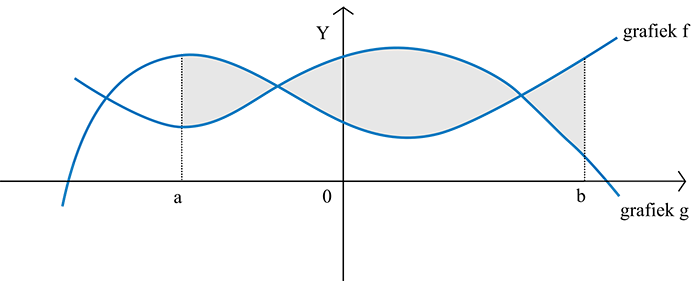
\includegraphics[width=0.7\linewidth]{6_afgeleiden_integralen/inputs/integraal3.png}
%	\caption{Berekenen van de oppervlakte tussen de grafieken van $f(x)$ en $g(x)$.}
%	\label{fig:integraal3}
%\end{figure}

\textbf{Methode:}

\begin{itemize}
	\item Maak een schets.
	\item Bepaal de grenzen van het interval welke het gebied begrenzen. Wanneer je de oppervlakte van het gebied bepaald door twee krommen wil bereken, zoek je de snijpunten van de krommen.
	\item Duid door middel van een rechthoekje een infinitesimaal klein deeltje aan. Duid op de figuur de breedte en de hoogte van het rechthoekje aan.
	\item Maak de som van de "deelintegralen". Elke deelintegraal stelt een oppervlakte voor en moet positief zijn.
	\item Oppervlakte gebied begrensd door $y=f(x)$ en  $y=g(x)$:
	\begin{equation*}
	S=\int_{x_2}^{x_1} |f(x)-g(x)| \dx
	\end{equation*}
\end{itemize}


\begin{voorbeeld}
	Bereken de oppervlakte tussen de rechte $y=x$ en de parabool $y=x^2$.
	
$y=x$: stijgende rechte door de oorsprong = $1^{\text{ste}}$ bissectrice.

$y=x^2$: dalparabool met top in de oorsprong en de $y$-as als symmetrieas.

Om de krommen te kunnen schetsen zoek je best nog enkele punten die voldoen aan de vergelijking. De punten vind je hier door in de vergelijking willekeurige -waarden in te vullen en de bijhorende -coördinaat te berekenen.

Hierboven zie je de grafiek van beide functies. De oppervlakte die we wensen te berekenen is de oppervlakte tussen de twee krommen. De verticale strookjes zullen dus moeten vertrekken van het eerste snijpunt en moeten stoppen bij het tweede snijpunt. Dit zijn de onder- en bovengrenzen van de integraal.

De hoogte van het strookje is $x-x^2$, de breedte is $\dx$, de oppervlakte van het rechthoekje is dan: 
We bepalen nu de grenzen van de integraal: dit zijn de $x$-waarden van de snijpunten van de parabool en de rechte, waar tussen de verticale strookjes gelegen zijn.

Om deze snijpunten te vinden, lossen we de volgende vergelijking op:
\begin{equation*}
x=x^2 \iff x-x^2=0 \iff x(1-x)=0
\end{equation*}
De $x$-waarden van de snijpunten zijn dus: $x=0$ en $x=1$. 
De oppervlakte van het gebied tussen de parabool en de rechte vinden we dan door de volgende integraal:
\begin{equation*}
\int_{0}^{1} (x-x^2)\dx = [\frac{x^2}{2}-\frac{x^3}{3}]_{x=0}^{x=1}=\frac{1}{2}-\frac{1}{3}=\frac{1}{6}
\end{equation*}
\end{voorbeeld}


\subsection{Test integralen}
%TODO